\newpage
\section{Versuchsaufbau und -durchführung}
  \subsection{Aufbau und Messvorbereitung}
    Der schematische Aufbau des hier genutzen Atomic Force Microscopes ist in Abbildung \ref{fig:Aufbau} dargestellt. Die Detektion erfolgt über das Lichtzeigerprinzip, indem ein sichtbarer Laser
    aus einer Glasfaser ausgekoppelt, auf den Cantilever gerichtet und dessen Reflektion von einer Vier-Segement-Diode detektiert wird. Der Cantilever kann starr befestigt werden, da das Abrastern und 
    Annähern zwischen Probe und Spitze über die Bewegung des Probentisches durch drei Piezoelemente für die Richtungen x, y und z erreicht wird. Die Bewegung der z-Piezo-Einheit wird über einen 
    PID-Controller gesteuert, der das Feedback der Vier-Segement-Diode berücksichtigt. Die ausgelesenen Daten werden auf einem Computer gespeichert und grafisch dargestellt.
    Um eine Probe zu untersuchen, wird der Probentisch manuell auf circa einen Centimeter von der Spitze entfernt und die Probe anschließend auf den Probentisch gelegt. Anschließend wird der Probentisch
    erneut manuell über Justierschrauben an die Spitze angenähert, bis die Spitze eine Auslenkung erfährt. Von diesem Punkt an übernimmt der Comoputer die Steuerung der Piezoelemente und hält den Abstand 
    zwischen Spitze und Probe konstant. Per Hand wird der Abstand nachgeregelt, bis das z-Piezoelement in neutraler Position ist und so eine maximale Auslenkung in beide Richtung möglich ist.
    \FloatBarrier
    \begin{figure}[h]
      \centering
      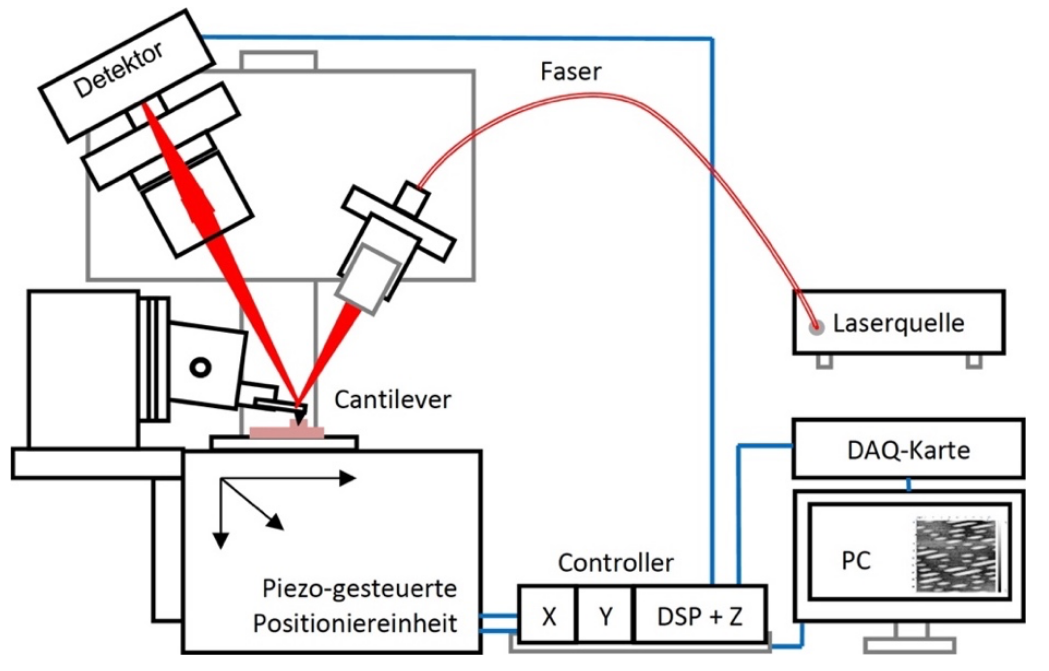
\includegraphics[width = 0.6\textwidth]{pictures/Aufbau.png}
      \caption{Der schematische Aufbau des Atomic Force Microscopes. Entnommen aus \cite{tu_dortmund_versuchsanleitung_nodate}}
      \label{fig:Aufbau}
    \end{figure}
    \FloatBarrier

  \newpage
  \subsection{Untersuchung einer Mikrostrukturprobe}
    Zunächst soll eine \SI{500}{\micro\metre}x\SI{1000}{\micro\metre} Probe untersucht werden, auf der, wie in Abbildung \ref{fig:Mikrostruktur} zu sehen, verschiedene Mikrostrukturen vorhanden sind.
    Die Kreis-, Streifen und Quadratstruktur werden alle in einem Bereich von \SI{20}{\micro\metre}x\SI{20}{\micro\metre} mit einer Auflösung von 250x250 Pixeln und einer Scan-Geschwindigkeit von 
    100 Pixeln/s im Constant-Force-Modus abgerastert. Während die Kreisstruktur mit eingeschalteter und ausgeschalteter Strain-Gauge-Nachregelung vermessen wird, werden die anderen Strukturen nur mit eingeschalteter 
    Strain-Gauge.Nachregelung vermessen. Um vor der tatsächlichen Messung die Orientierung der Probe zu überprüfen, werden schnelle Scans mit niedriger Auflösung durchgeführt.

    \begin{figure}[h]
      \centering
      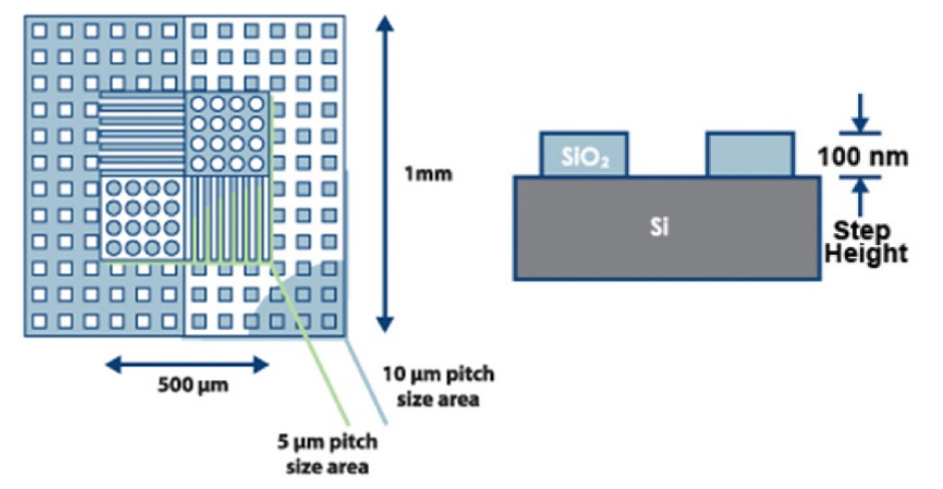
\includegraphics[width = 0.6\textwidth]{pictures/Mikrostruktur.png}
      \caption{Abbildung der zu vermessenden Mikrostruktur von oben betrachtet (links) und im Querschnitt (rechts). Entnommen aus \cite{tu_dortmund_versuchsanleitung_nodate}}
      \label{fig:Mikrostruktur}
    \end{figure}
    \FloatBarrier
  \subsection{Untersuchung einer CD, DVD und Bluray}
    Um die Absenkungen in den Disc-Speichermedien zu vermessen, werden Stücke einer CD, DVD und Bluray ausgeschnitten und ebenfalls vermessen. Da die Absenkungen für die Discs mit größeren Speicherkapazitäten
    immer kleiner werden, müssen auch die Scanparameter auf höhere Genauigkeit angepasst werden. Für die Messungen, die im Constant-Force-Modus durchgeführt werden, werden daher, die in Tabelle 
    \ref{tab:Scanparameter} aufgetragenen Scanparameter verwendet.

    \begin{center}
      \captionof{table}{Scanparameter}
      \label{tab:Scanparameter}
      \begin{tabular}{c c c c}
          \toprule
          Probe & Scanbereich & Auflösung & Scangeschwindigkeit \\
          \midrule
          CD      & \SI{10}{\micro\metre} x \SI{10}{\micro\metre} & 250 x 250 Pixel & 100 Pixel/s \\
          DVD     & \SI{5}{\micro\metre} x \SI{5}{\micro\metre}   & 250 x 250 Pixel & 100 Pixel/s \\
          Bluray  & \SI{2}{\micro\metre} x \SI{2}{\micro\metre}   & 250 x 250 Pixel & 50 Pixel/s \\

          \bottomrule
      \end{tabular}
  \end{center}
